\begin{frame}{Liste des concepts médicaux}
Extraction semi-automatique des termes en lien avec Charcot.\\~\\

 \begin{figure}[!htb]
    \centering
    \begin{minipage}{.5\textwidth}
        \centering
        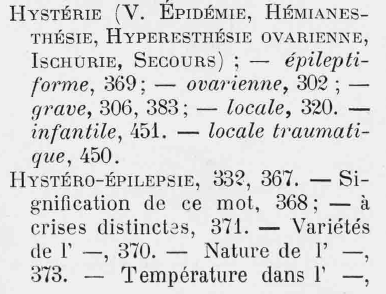
\includegraphics[width=0.6\linewidth, height=0.3\textheight]{pic/concepts-pdf}
        \caption{Index des termes \citep{charcot1890oeuvres}.}
        \label{fig:prob1_6_2}
    \end{minipage}%
    \begin{minipage}{.5\textwidth}
        \centering
        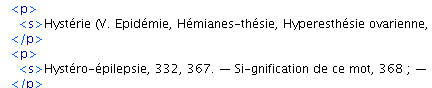
\includegraphics[width=1\linewidth, height=0.15\textheight]{pic/concepts-xml}
        \caption{Concepts médicaux, document XML.}
        \label{fig:prob1_6_1}
    \end{minipage}
\end{figure}
%\begin{figure}[!h]
%    \centering
%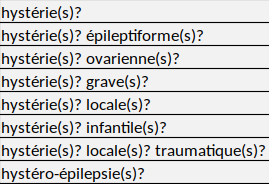
\includegraphics[width=30mm,scale=0.5]{pic/concepts-csv.png}
%\caption{Liste finale des concepts médicaux.}
%    \label{fig:my_label}
%\end{figure}
 \begin{figure}[!htb]
    \centering
    \begin{minipage}{.5\textwidth}
        \centering
        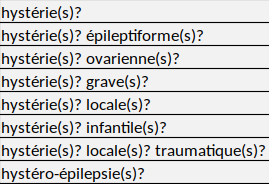
\includegraphics[width=0.6\linewidth, height=0.25\textheight]{pic/concepts-csv}
        \caption{Liste finale des concepts médicaux.}
        \label{fig:prob1_6_2}
    \end{minipage}%
    \begin{minipage}{.6\textwidth}
        \centering
   \begin{enumerate}
   \setcounter{enumi}{3}
   \item entre \texttt{<s>} et \texttt{,-(} (regex)
   \item sans termes génériques (\textit{os}, \textit{peau})
\item prise en compte des sg. / pl. (regex)
   \end{enumerate}
    \end{minipage}
\end{figure}
\end{frame}

\begin{frame}{Calcul de pertinence des concepts}
Trois mesures de pondération : \textsc{TF-IDF}, \textsc{BM25} et \textsc{BERT}.
    \footnotesize
\begin{table}[]
\begin{tabular}{|l|cccc|}
\hline
\multicolumn{1}{|c|}{\multirow{}{}{Terme}} & \multicolumn{4}{c|}{\cellcolor{gray!10!white}{ Corpus \og{}Autres\fg{}}}                              \\ \cline{2-5} 
\multicolumn{1}{|c|}{}                       & \multicolumn{1}{c}{{Fréquence}} & \multicolumn{1}{c}{{TF-IDF}} & \multicolumn{1}{c}{{BM25}}  & {BERT} \\ \hline
{Arthrite déformante} &
  \multicolumn{1}{|r|}{{24}} &
  \multicolumn{1}{|r|}{{0,02}} &
  \multicolumn{1}{|r|}{{0,50}} &
  {0,40} \\ \hline
{Ataxie locomotrice} &
  \multicolumn{1}{|r|}{{169}} &
  \multicolumn{1}{|r|}{{0,08}} &
  \multicolumn{1}{|r|}{{0,25}} &
  {0,39} \\ \hline
{Atrophie musculaire} &
  \multicolumn{1}{|r|}{{1465}} &
  \multicolumn{1}{|r|}{{0,43}} &
  \multicolumn{1}{|r|}{{0,15}} &
  {0,42} \\ \hline
{Atrophie progressive} &
  \multicolumn{1}{|r|}{{22}} &
  \multicolumn{1}{|r|}{{0,02}} &
  \multicolumn{1}{|r|}{{0,53}} &
  {0,39} \\ \hline
{Catalepsie} &
  \multicolumn{1}{|r|}{{975}} &
  \multicolumn{1}{|r|}{{0,28}} &
  \multicolumn{1}{|r|}{{0,15}} &
  {0,39} \\ \hline
{Épilepsie} &
  \multicolumn{1}{|r|}{{577}} &
  \multicolumn{1}{|r|}{{0,12}} &
  \multicolumn{1}{|r|}{{0,10}} &
  {0,41} \\ \hline
{Hystérie} &
  \multicolumn{1}{|r|}{{4934}} &
  \multicolumn{1}{|r|}{{0,45}} &
  \multicolumn{1}{|r|}{{0,05}} &
  {0,41} \\ \hline
{Langue} &
  \multicolumn{1}{|r|}{{3591}} &
  \multicolumn{1}{|r|}{{0,11}} &
  \multicolumn{1}{|r|}{{0,02}} &
  {0,41} \\ \hline
{Maladie de Parkinson} &
  \multicolumn{1}{|r|}{{130}} &
  \multicolumn{1}{|r|}{{0,09}} &
  \multicolumn{1}{|r|}{{0,35}} &
  {0,37} \\ \hline
{Paralysie bulbaire} &
  \multicolumn{1}{|r|}{{93}} &
  \multicolumn{1}{|r|}{{0,09}} &
  \multicolumn{1}{|r|}{{0,52}} &
  {0,40} \\ \hline
{Paralysie rhumatismale} &
  \multicolumn{1}{|r|}{{14}} &
  \multicolumn{1}{|r|}{{0,02}} &
  \multicolumn{1}{|r|}{{0,68}} &
  {\cellcolor{green!30!white}{\textcolor{purple}{\textbf{0,44}}}} \\ \hline
{Sclérose latérale} &
  \multicolumn{1}{|r|}{{127}} &
  \multicolumn{1}{|r|}{{0,09}} &
  \multicolumn{1}{|r|}{{0,37}} &
  {0,41} \\ \hline
{Sclérose en plaque disséminées} &
  \multicolumn{1}{|r|}{{12}} &
  \multicolumn{1}{|r|}{{0,02}} &
  \multicolumn{1}{|r|}{\cellcolor{green!30!white}{\textcolor{purple}{\textbf{0,83}}}} &
  {0,40} \\ \hline
{Somnambulisme} &
  \multicolumn{1}{|r|}{{3410}} &
  \multicolumn{1}{|r|}{\cellcolor{green!30!white}{\textcolor{purple}{\textbf{1}}}} &
  \multicolumn{1}{|r|}{{0,15}} &
  {0,43} \\ \hline
\end{tabular}
\caption{Pertinence des concepts sous forme des scores TF-IDF, BM25 et BERT, corpus \og{}Autres\fg{}.}
\end{table}
\end{frame} 

\begin{frame}{Intensification du discours
de Charcot dans le corpus \textrm{Autres}}
Le terme le plus impactant pour le réseau de Charcot selon \textsc{BM25} :\\
\textit{sclérose en plaque disséminées} ? (pertinence : 83\%)
\begin{figure}[!h]
    \centering
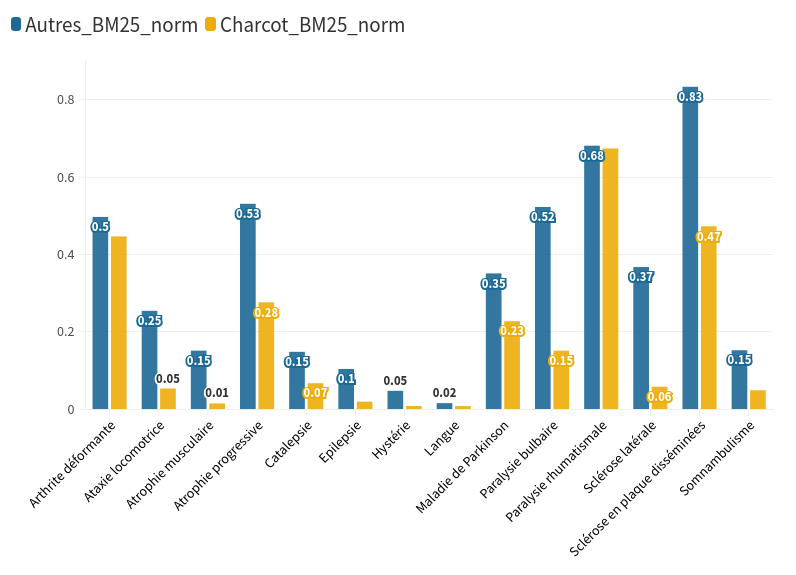
\includegraphics[width=80mm,scale=0.5]{pic/Charcot_Autres_250523.png}
    \caption{Pertinence des concepts dans les deux corpus (BM25).}
    \label{fig:my_label}
\end{figure}
\end{frame}

\begin{frame}{\textsc{BERT}}
\cite{vaswani2021}
    \begin{itemize}
        \item plongements lexicaux et des
mécanismes d’attention
        \item modèle \texttt{bert-base-multilingual-cased}
    \end{itemize}

\begin{table}[]
\begin{tabular}{|ll|ll|}
\hline
\multicolumn{2}{|c|}{\cellcolor[HTML]{EFEFEF}Corpus \og{}Charcot\fg{}} & \multicolumn{2}{c|}{\cellcolor[HTML]{EFEFEF}Corpus \og{}Autres\fg{}}     \\ \hline
\multicolumn{1}{|l|}{diplopie}                & 0,92 & \multicolumn{1}{l|}{préambule}       & 0,47      \\
\multicolumn{1}{|l|}{myélite partielle}       & 0,91 & \multicolumn{1}{l|}{délire}          & 0,47      \\
\multicolumn{1}{|l|}{état de mal épileptique} & 0,91 & \multicolumn{1}{l|}{miracle}         & 0,47      \\
\multicolumn{1}{|l|}{paralysie labio-glosso-laryngée} & 0,91 & \multicolumn{1}{l|}{cicatrices vicieuses} & 0,46 \\ \hline
\multicolumn{2}{|c|}{\cellcolor[HTML]{E1FFE1}\textsc{pathologies}}     & \multicolumn{2}{c|}{\cellcolor[HTML]{FFDFDD}\textsc{notions abstraites}} \\ \hline 
\end{tabular}
\end{table}
\end{frame}